\documentclass[nocfonts,fleqn,folios]{deutschesmuseum}
\usepackage{kantlipsum, booktabs, graphicx}
\begin{document}
\title{Typographical samples}
\subtitle{Sample file for Deutsches Museum}
\author{Boris Veytsman \and C.~O.~Respondent}
\maketitle

\begin{abstract}
  This is a demo for the Deutsches Museum contribution style.
\end{abstract}

\section{Introduction}
\label{sec:intro}

We can have numbered sections.  Quotations, for
example\cite[][Article~7]{UNDeclaration}: 
\begin{quote}
  All are equal before the law and are entitled without any
  discrimination to equal protection of the law. All are entitled to
  equal protection against any discrimination in violation of this
  Declaration and against any incitement to such discrimination. 
\end{quote}

\subsection{Subsection example}
\label{sec:subsection}

We can have subsections and footnotes\footnote{A normal footnote}.

\section{Mathematics}
\label{sec:math}

The samples below are based on the example from the \emph{Free Math
  Fonts Survey}\cite{Hartke06,
  free-math-font-survey}.


\textbf{Theorem 1 (Residue Theorem).}
Let $f$ be analytic in the region $G$ except for the isolated singularities $a_1,a_2,\ldots,a_m$. If $\gamma$ is a closed rectifiable curve in $G$ which does not pass through any of the points $a_k$ and if $\gamma\approx 0$ in $G$ then
\[
\frac{1}{2\pi i}\int_\gamma f = \sum_{k=1}^m n(\gamma;a_k) \text{Res}(f;a_k).
\]

\textbf{Theorem 2 (Maximum Modulus).}
\emph{Let $G$ be a bounded open set in $\mathbb{C}$ and suppose that $f$ is a continuous function on $G^-$ which is analytic in $G$. Then}
\[
\max\{|f(z)|:z\in G^-\}=\max \{|f(z)|:z\in \partial G \}.
\]

Maxwell's equations
\begin{align}
  \nabla\cdot\mathbf{E} &= \frac{\rho}{\epsilon_0}\\
  \nabla\cdot\mathbf{B} &= 0\\
  \nabla\times\mathbf{E} &= - \frac{\partial\mathbf{B}}{\partial t}\\
  \nabla\times\mathbf{B} &= \mu_0\left(
                           \mathbf{J} +
                           \epsilon_0\frac{\partial\mathbf{E}}{\partial
                           t}
                           \right).
\end{align}

We also can have figures (Fig.~\ref{fig:vitruvian}) and tables
(Table~\ref{tab:one}).  

\begin{figure}
  \centering
  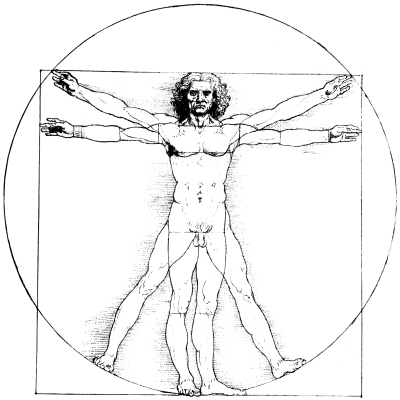
\includegraphics{vitruvian}
  \caption{Vitruvian man}
  \label{fig:vitruvian}
\end{figure}

\begin{table}
  \caption[Sed blandit, tortor a auctor]{Sed blandit, tortor a auctor
    imperdiet, wisi nibh ornare leo, 
    ac dictum nibh enim eu orci}
  \begin{tabular}{lll}
    \toprule
    \bfseries Phasellus &  \bfseries At Dui       & \bfseries Donec Commodo \\
    \midrule    
     Augue At Nunc    & Nunc In  sapien       & Et magna mollis \\
     Sagittis         &  Morbi eu elit        &  Phasellus lacus\\
     Donec a quam     & Etiam pulvinar sapien & Sed nibh magna\\
    \bottomrule
  \end{tabular}
\label{tab:one}
\end{table}


\section{Some pseudo-Kant}
\label{sec:kant}


We are using \textsl{kantlipsum} package\cite{kantlipsum}. 

\kant[1-25]



\bibliographystyle{plainnat}
\bibliography{sample}

\end{document}
